%%%%%%%%%%%%%%%%%%%%%%%%%%%%%%%%%%%%%%%%%%%%%%%%%%%
%% P3: Phenomenology of Particle Physics                         
%%
%% Author:  André Rubbia                   		 
%%
%% Figure 5.7 Kinematics of $\pi^0\rightarrow \gamma\gamma$ relative to center-of-mass (left) and laboratory frame (right).
%%
%% This work is licensed under the Creative Commons Attribution 4.0 International License. 
%% To view a copy of this license, visit http://creativecommons.org/licenses/by/4.0/ or 
%% send a letter to Creative Commons, PO Box 1866, Mountain View, CA 94042, USA.
%%
%%%%%%%%%%%%%%%%%%%%%%%%%%%%%%%%%%%%%%%%%%%%%%%%%%%

\documentclass[a4paper,10pt]{article}

\usepackage[T1]{fontenc}
\usepackage[utf8]{inputenc}
\usepackage{lmodern}
\usepackage[labelfont=bf]{caption}
\usepackage{upgreek}

\usepackage{tikz}
\usepackage{pgfplots}
\pgfplotsset{compat=1.17}
\usepgfplotslibrary{ternary}
\usepgfplotslibrary{fillbetween}
\usepgfplotslibrary{external}
\usetikzlibrary{patterns}
\usetikzlibrary{decorations.pathmorphing}
\usetikzlibrary{decorations.markings}
\usetikzlibrary{arrows}
\usetikzlibrary{svg.path}
\usetikzlibrary{shapes}
\usetikzlibrary{arrows.meta}
% define the arrow style
\tikzset{
    arrow/.style={
        decoration={
            markings,
            mark=at position .5 with {
                \arrow[#1, scale=1.5]{latex}
            }
        },
        postaction={decorate},
    }
}
\tikzset{
    arrow flipped/.style={
        decoration={
            markings,
            mark=at position .5 with {
                \arrow[#1, scale=1.5]{latex reversed}
            }
        },
        postaction={decorate},
    }
}
\pgfkeys{/pgf/number format/.cd,1000 sep={}}\usepackage{pgfplots}

\def\d{\mathrm{d}}

\begin{document}

%%%%%%%%%%%%%%%%   FIGURE  %%%%%%%%%%%%%%%%%%%%%%%%%%%%%%
\begin{figure}[htb]
\begin{center}
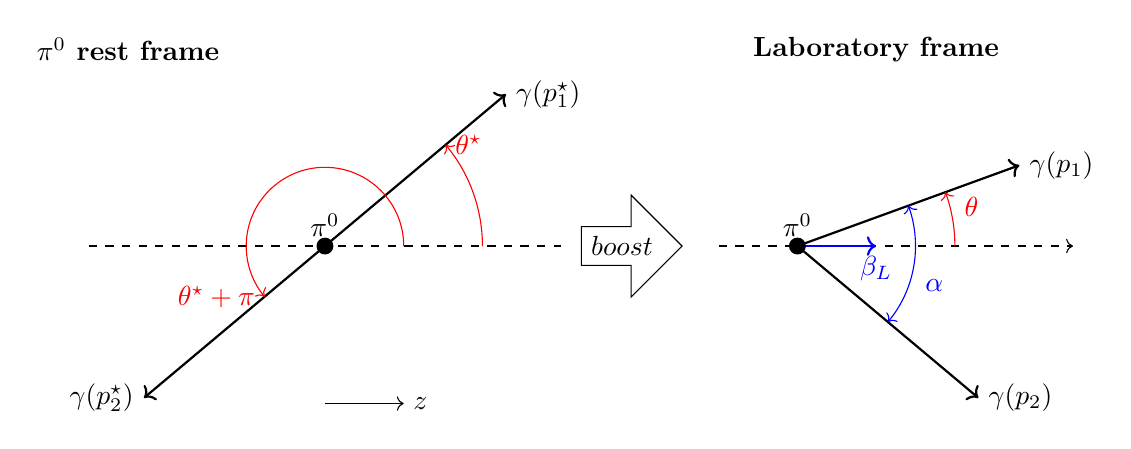
\begin{tikzpicture}
\draw[dashed] (-3.,0) -- (3.,0);

\node[draw, single arrow,
              minimum height=10mm, minimum width=8mm,
              single arrow head extend=4mm,
              anchor=west, rotate=0] at (3.25,0) {$boost$};

\filldraw (0,0) circle (1mm) node [above] {$\pi^0$};
\draw[thick,->] (0,0) -- +(40:3) node [right] {$\gamma(p^\star_1)$};
\draw[thick,->] (0,0) -- +(220:3) node [left] {$\gamma(p^\star_2)$};
\draw[red,->] (2,0) arc(0:40:2) node [right] {$\theta^\star$};
\draw[red,->] (1,0) arc(0:220:1) node [left] {$\theta^\star+\pi$};
\node at (-2.5,2.5) {\textbf{$\pi^0$ rest frame}};
\draw[dashed,->] (5,0) -- (9.5,0);
\draw[thick,blue,->] (6,0)--+(0:1) node [below] {$\beta_L$};
\node at (7,2.5) {\textbf{Laboratory frame}};
\filldraw (6,0) circle (1mm) node [above] {$\pi^0$};
\draw[thick,->] (6,0) -- +(20:3) node [right] {$\gamma(p_1)$};
\draw[thick,->] (6,0) -- +(-40:3) node [right] {$\gamma(p_2)$};
\draw[red,->] (8,0) arc(0:20:2);
\node[red] at (8,0.5) [right] {$\theta$};
\draw[blue,->] (7.5,0) arc(0:20:1.5);
\draw[blue,->] (7.5,0) arc(0:-40:1.5);
\node[blue] at (7.5,-0.5) [right] {$\alpha$};
\draw[->] (0,-2) -- +(0:1) node[right] {$z$};
\end{tikzpicture}
\caption{Kinematics of $\pi^0\rightarrow \gamma\gamma$ relative to center-of-mass (left) and laboratory frame (right). The \textbf{opening angle $\alpha$}
between the two photons in the laboratory frame is also shown.}
\end{center}
\end{figure}
%%%%%%%%%%%%%%%%   END FIGURE  %%%%%%%%%%%%%%%%%%%%%%%%%%%%%%

\end{document}
